\documentclass{article}

\usepackage{lipsum}
\usepackage[margin=1in,includefoot]{geometry}
\usepackage{graphicx}
\usepackage{float}
\usepackage[hidelinks]{hyperref}
\usepackage{amsmath}
\usepackage{amssymb}
\usepackage{color}


\usepackage[usenames,dvipsnames]{xcolor}
\usepackage{listings}
\lstset {language=C++}






% Header and Footer Stuff
\usepackage{fancyhdr}
\pagestyle{fancy}
\fancyhead{}
\fancyfoot{}
\fancyfoot[R]{\thepage}
\renewcommand{\headrulewidth}{0pt}
\renewcommand{\footrulewidth}{0pt}


\definecolor{dkgreen}{rgb}{0,0.6,0}
\definecolor{gray}{rgb}{0.5,0.5,0.5}
\definecolor{mauve}{rgb}{0.58,0,0.82}

\lstset{
  language=VHDL,
  aboveskip=3mm,
  belowskip=3mm,
  showstringspaces=false,
  columns=flexible,
  basicstyle={\small\ttfamily},
  numbers=none,
  numberstyle=\tiny\color{gray},
  keywordstyle=\color{blue},
  commentstyle=\color{dkgreen},
  stringstyle=\color{mauve},
  breaklines=true,
  breakatwhitespace=true,
  tabsize=3
}


\begin{document}

\begin{titlepage}
	\begin{center}
	\begin{align*}
	
\includegraphics[height=1.75in]{logo.png}
	\end{align*}


	
	\line(1,0){300}\\
	[0.25in]
	\huge{\bfseries Tutorial 1 }\\
	[2mm]
	\line(1,0){200}\\
	[1.5cm]
	\textsc{\LARGE Triangles}\\
	[0.75cm]
	\textsc{\Large CS4052 Computer Graphics}\\
	[7cm]	
	\end{center}
	
	
	
	\begin{flushright}
	\textsc{\large Alexandru Sulea\\
	D Stream\\
	\#12315152\\
	27 September 2016\\}
	\end{flushright}
	
\end{titlepage}
%Table of Contents Stuff%
%\tableofcontents
%\listoffigures
%\addcontentsline{toc}{section}{List of Figures}
%\listoftables
%\addcontentsline{toc}{section}{List of Tables}


\thispagestyle{empty}
\cleardoublepage
\pagenumbering{arabic}
\setcounter{page}{1}

\pagebreak
\section{Making a Coloured Triangle}
I called the buffer by the color preset variable name which coloured the triangle with the preset color gradient
\begin{lstlisting}
// Fragment Shader
// Note: no input in this shader, it just outputs the colour of all fragments, in this case set to red (format: R, G, B, A).
static const char* pFS = "                                              \n\
#version 330                                                            \n\
/*since FeagColor5 is an out vector, its name does not need to corespond to anything \n\
this is onl required for the possible out vecttor FragColor	*/		 \n\
out vec4 FragColor5;                                                      \n\
/*for future reference make sure mapping and shading names are the same*/     \n\
in vec4 color;																\n\
void main()                                                               \n\
{                                                                          \n\
FragColor5 =  vec4(color);	}";
\end{lstlisting}
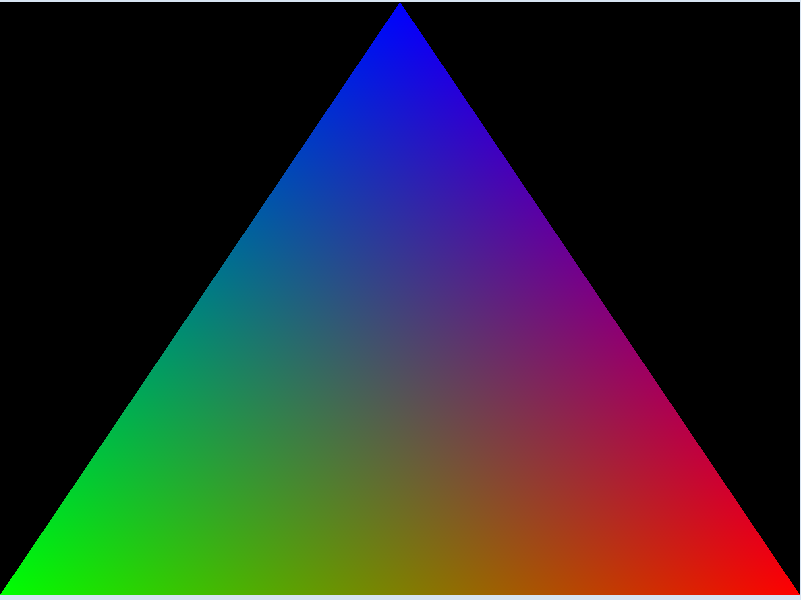
\includegraphics[height=1.75in]{triangle.PNG}


\section{Making the triangle twice as small}
Since I wasnt allowed to alter the vertices array I divided everything by 2
\begin{lstlisting}
void main()                                             \n\
{                                                       \n\
    gl_Position = vec4(vPosition.x/2, vPosition.y/2, vPosition.z/2, 1.0);  \n\
	color = vColor;							\n\}";
\end{lstlisting}
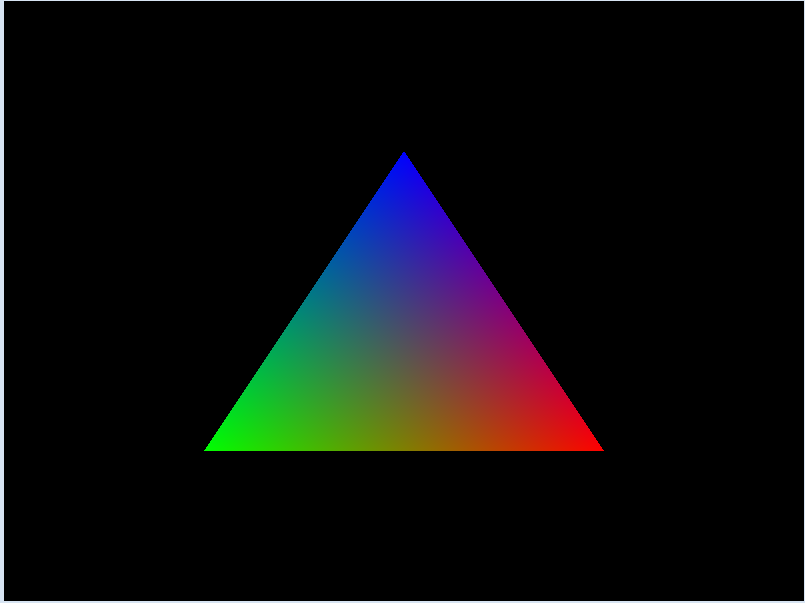
\includegraphics[height=1.75in]{triangle_5.PNG}
\pagebreak
\section{Making a red and yello square}
I drew another triangle and extended the original one by adding extravertices.\\
I also added new color coordinates for the new vertices\\
I looked up the color for red and yellow so as to map the points appropriatelly.\\
I changed the number of vertices in the display and mapping functions.\\

\begin{lstlisting}
	GLfloat vertices[] = { 
		1.0f, -1.0f, 0.0f,
		1.0f, 1.0f, 0.0f,
		-1.0f, 1.0f, 0.0f,

		-1.0f, 1.0f, 0.0f,
		-1.0f, -1.0f, 0.0f,
		 1.0f, -1.0f, 0.0f};
GLfloat colors[] = {1.0f, 1.0f, 0.0f, 1.0f,   
						1.0f, 0.0f,0.0f,  1.0f,   
						1.0f, 1.0f, 0.0f, 1.0f, 

						1.0f, 1.0f, 0.0f, 1.0f,
						1.0f, 0.0f,0.0f,  1.0f,    
						1.0f, 1.0f, 0.0f, 1.0f};
					
		GLuint numVertices = 6;
\end{lstlisting}


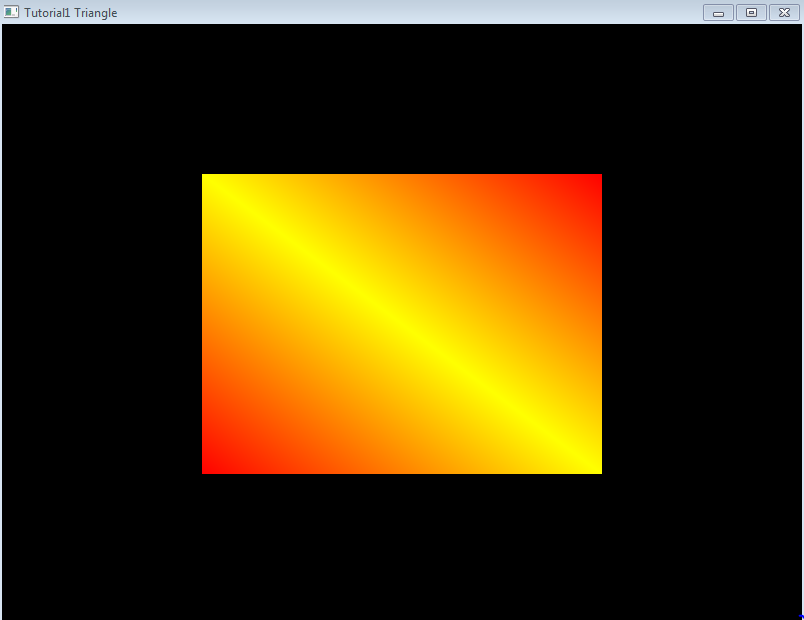
\includegraphics[height=1.75in]{square.PNG}


\pagebreak

	
\end{document}